
\likechapter{Введение}
\todo[inline, color=red]{2-3 страницы пока не понятно о чем???}
\chapter{Автоматизация производственного планирования}
\section{Система управления и планирования предприятием}
На сегодняшний день, в условиях серьезной конкуренции очень важно следить за всеми новинками технологического прогресса и своевременно внедрять в структуру производства.
Так организация предприятия напрямую влияет на эффективность производства. Основным направлением организацией предприятием в последнее время относят системы ИСУП, которые позволяют достичь следующих задач: выполнение планов производства, оптимизация производственного процесса, снижение издержек и повышение эффективности производства.

Данные системы начали появляться с развитием компьютерных технологий в начале 80-х годов. Одной из главных причин появления данных систем является нехватка административного, бухгалтерского и технического персонала, который обладал бы достаточной квалификацией для обработки информации предприятия, также стало понятно, что предприятия не могут позволять себе большие объемы материального запаса для производства продукции. Это привело к появлению систем планирования потребности в ресурсах. Первым шагом в этом направлении был MRP (Materials Resource Planning), который включал только материалы планирования для производства [7].

Основной концепция MPR заключается в минимизации затрат связанных с запасами, а также расчет сколько и в какие сроки необходимо произвести конечный продукт. 

Недостатками данной системы является, то что при расчете потребностей в материалах не учитываются производственные мощности, их загрузки, трудозатраты и т.д. 

Логическим продолжением MPR системы стала система MPR 2, которая в отличие от предшественника учитывала финансовую составляющую предприятия, а также охватывала более широкий охват ресурсов. Это позволило компаниям иметь более интегрированную бизнес-систему, которая выводила требования к материалам и мощности, связанные с желаемым планом операций, позволяла вводить подробные данные о деятельности, переводить все это в финансовый отчет и предложить план действий для решения тех вопросов, которые были не в соответствии с желаемым планом.

К началу 1990-х годов постоянные улучшения в технологии позволили расширить MRP II, включив в него все планирование ресурсов для всего предприятия. Такие области, как дизайн продукта, хранение информации, планирование мощностей, системы связи, управление персоналом, финансы и управление проектами, теперь могут быть включены в план. Отсюда и термин ERP (Enterprise Resource Planning). И ERP можно использовать не только в производственных компаниях, но и в любой компании, которая хочет повысить конкурентоспособность путем наиболее эффективного использования всех своих активов, включая информацию [23,25].

Разрабатываемое программное обеспечение принадлежит к классу ERP-систем. Многие современные ERP-систем разработаны по модульному принципу, поэтому существует возможность выбирать и внедрять только те модули, которые необходимы клиенту. 

В данной работе рассматривается одна из частей ERP систем,отвечающая за сопоставление конструкторских и технологических спецификаций, определяющих состав конечного продукта и ресурсов предприятия. На основании данного сопоставления построение плана производственного процесса, учитывающие ограничения предприятия, а также реализация частных математических моделей. Математические модели призваны оптимизировать производственный процесс в зависимости от специфики предприятия( конвейерное производство ).


\section{Источники роста эффективности}

В промышленности есть огромные неиспользованные резервы роста производительности труда. Они могут быть подразделены на резервы снижения трудоемкости продукции и резервы рабочего времени.( см. рисунок \ref{ris:reserve1})

Резервы снижения трудоемкости выявляются и реализуются в виде экономии рабочего времени, затрачиваемого непосредственно на выполнение рабочих операций.

Резервы фонда рабочего времени реализуются путем повышения эффективности использования рабочего процесса для данного коллектива в течение определенного планового периода. 


\begin{figure}[H]
    \center{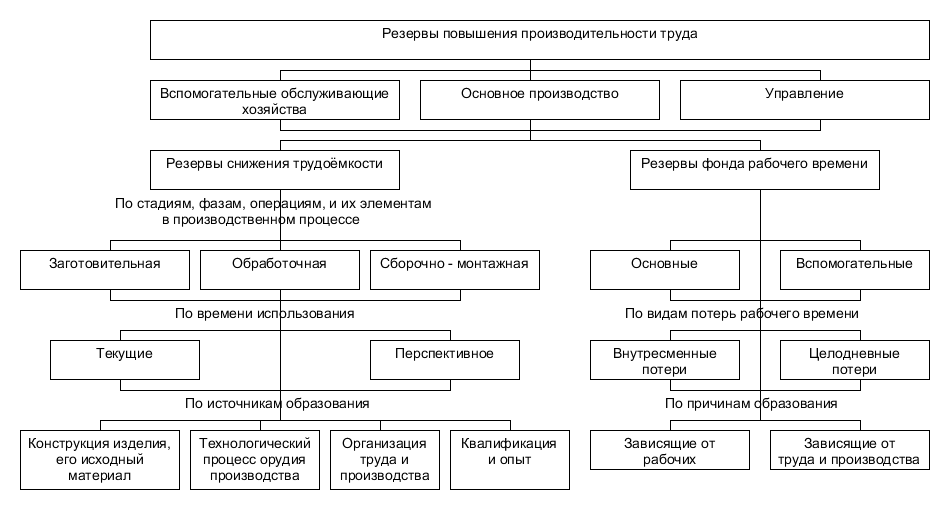
\includegraphics[width=1\linewidth]{fig/reserve1.png}}
    \caption{Резервы роста производительности труда}
    \label{ris:reserve1}
\end{figure}

Исходя из информации представленной на рисунке \ref{ris:reserve1}, можно сделать вывод, что повышение эффективности производства может быть достигнуто, как и грамотной организацией резервов рабочего времени, так и путем пересмотра техники выполнения рабочих операций, но не все резервы повышения производительности можно решить в рамках ИУС. К таким резервам относится конструктивные особенности изделия, так как требуют изменения исходной конструкции продукта, что не является задачей ИУС. 

\section{Обзор методов планирования производственных процессов.}
\subsection{Объемный метод планирования}
\subsection{Календарный метод планирования}
\subsection{Объемно-календарный метод планирования}
\subsection{Объемно-динамический метод планирования}
\section{Постановка задачи}
Цель работы: повышение производительности труда на сборочных производствах за счет автоматизации и оптимизации процессов планирования.

Задачи: 
\begin{itemize}
    \item Обзор методов и средств повышения производительности труда.
    \item Разработка математической модели планирования
    \item Разработка архитектуры ПО
    \item Разработка алгоритмов оптимизации плана работы на такт
    \item Прототипирование
\end{itemize}

\chapter{Теоретическая часть}

\section{Архитектура ПО}

\begin{figure}[H]
    \center{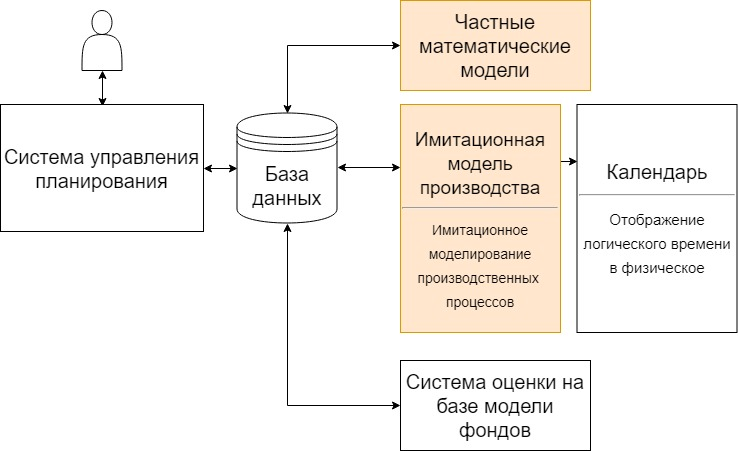
\includegraphics[width=1\linewidth]{fig/arh1.jpg}}
    \caption{Архитектура ПО}
    \label{ris:arh1}
\end{figure}

На рисунке \ref{ris:arh1} представлена архитектуры программного обеспечения. Данная архитектура содержит следующие элементы:

\begin{itemize}
    \item пользовательский интерфейс для взаимодействия с системой, который также позволяет получать информацию о работе системы в виде диаграмм, или графиков; 
    \item система управления планирования взаимодействует со всеми элементами системы и является главным распорядителем задач;
    \item база данных хранит всю информацию о производстве и результаты планирования; 
    \item имитационная модель производства создает план на основе информации из технологической карты и производственного плана;
    \item календарь обрабатывает абсолютные значения, используемые при планировании, и привязывает их к конкретным датам;
    \item частные оптимизационные модели работают с уже сформировавшимся планом, который получен в результате имитационного моделирования. К данному плану применяются алгоритмы оптимизации, зависящие от конкретных целей. Таким целями могут быть: задачи упорядочивания, задачи согласования, задачи распределения, задачи с суммарными критериями оптимизации, задачи с минимаксимальными критериями оптимизации[1, 2].
\end{itemize}

\section{Формализация постановки задачи}
Для того, чтобы разрабатывать алгоритмы планирования в первую очередь необходимо формализовать предметную область. В данном случае формализуется сборочный цех со значимыми внутренними особенностями.

Как правило на любом предприятии имеется специальный документ – технологическая карта, детально описывающая весь перечень операций по достижению которых воспроизводится единица продукции. Технологическая карта хранит информацию о зависимостях между операциями, привязках ресурсов к операциям, трудоёмкостях операций, периодичность операций, результат каждой операции. 

Далее важно учесть ресурсы предприятия. В рамках сборочного производства такими ресурсами могут быть: персонал, оборудование, организация конвейерной производственной линии.

Последним пунктом для построения модели производства является производственный план. То есть перечень продукции в составе заказа и срок реализации данного заказа. На рисунке \ref{ris:Prod1} представлен пример взаимодействия перечисленных выше моделей. 

\begin{figure}[H]
    \center{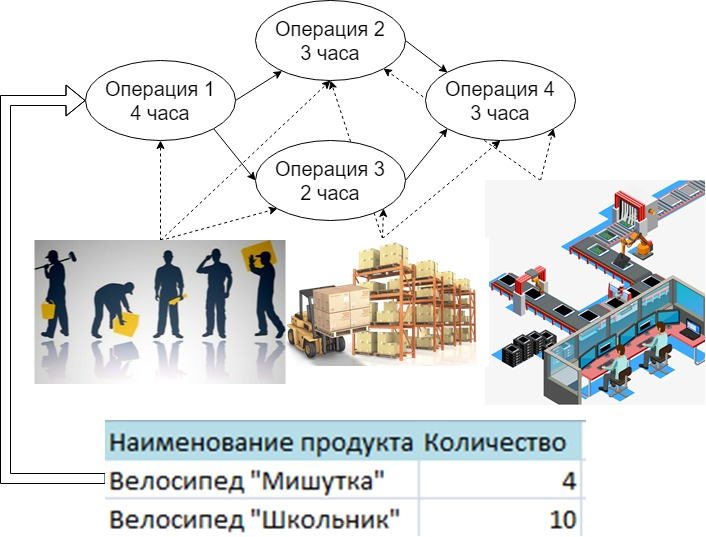
\includegraphics[width=1\linewidth]{fig/Prod1.jpg}}
    \caption{Модель производства}
    \label{ris:Prod1}
\end{figure}


\section{Математическое моделирование производственных процессов}

Для формализации процесса планирования в работе используются системы неравенств. Пример системы неравенств представлена на рисунке \ref{ris:sys1}. Система неравенств состоит из двух частей: статическую и динамическую. Статическая по своей сути копирует последовательность операций, описываемых в технологической карте. Динамическая накладывает дополнительные ограничения на систему неравенств, которая складывается из ресурсных зависимостей. Ресурсными зависимостями являются связи между операциями и фондом предприятия[3].

\begin{figure}[H]
    \center{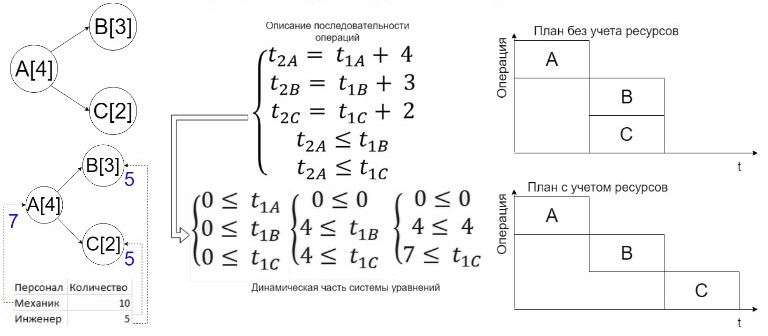
\includegraphics[width=1\linewidth]{fig/Screenshot_3.jpg}}
    \caption{Система неравенств}
    \label{ris:sys1}
\end{figure}

Таким образом планирование делится на шаги, каждый раз при этом формируются новые ограничения вводимые ресурсами[4].

\section{Балансировка сборочной линии}

Производственная сборочная линия была впервые представлена
Генри Форд в начале 1900-х годов. Она была разработана, чтобы быть эффективным,
высокопроизводительным способом изготовления конкретного продукта. Базовая сборочная
линия состоит из набора рабочих станций, расположенных линейно, где каждая станция соединена погрузочно-разгрузочным устройством.
Основное движение материала по сборочной линии начинается с того, что деталь подается на первую станцию с
заданной скоростью подачи. Станция считается любой точкой на конвейере, в которой 
выполняется задание с заготовкой. Эти задачи могут выполняться машинами, роботами и
или людьми. Как только деталь поступает на станцию, то для нее выполняется задание, 
и деталь подается на следующую операцию. Время, необходимое для выполнения задачи
в каждой операции, называется временем процесса (Sury, 1971). Время цикла сборочной 
линии определяется желаемой производительностью. Этот уровень производства 
устанавливается таким образом, чтобы желаемое количество конечного продукта 
производилось в течение определенного периода времени (Baybars, 1986). Для того чтобы 
сборочная линия поддерживала определенную производительность, сумма времени обработки
на каждой станции не должна превышать время цикла на станциях (Fonseca et al, 2005). 
Если сумма времен обработки внутри станции меньше времени цикла, говорят, что на этой
станции присутствует время простоя (Erel et al, 1998). Одним из основных вопросов,
касающихся разработки сборочной линии, является порядок организации задач, которые 
необходимо выполнить. Для изготовления любого предмета есть несколько 
последовательностей задач, которые необходимо выполнить. Проблема балансировки 
сборочной линии (ALBP) возникла с изобретением сборочной линии. Хельгесон и др. 
(Helgeson и др., 1961) были первыми, кто предложил ALBP, а Сальвесон (Salveson, 1955)
был первым, кто опубликовал проблему в ее математической форме. 
Однако в течение первых сорока лет существования сборочной линии для балансировки
линий использовались только методы проб и ошибок (Erel et al., 1998). С тех пор 
было разработано множество методов для решения различных форм ALBP. 
Сальвесон (Salveson, 1955) сделал первую математическую попытку, решив задачу в
виде линейной программы. Гутьяр и Немхаузер (Gutjahr и Nemhauser, 1964) показали,
что проблема ALBP относится к классу NP-сложных задач комбинаторной оптимизации.
Это означает, что оптимальное решение не гарантируется для задач значительных размеров. 
Поэтому эвристические методы стали наиболее популярными методами решения проблемы.


Преимущества балансировки линии:

\begin{itemize}
    \item Минимизация количества рабочих станций при заданном цикле
    \item Минимизация цикла при заданном количестве рабочих станций
    \item Минимизация общего времени простоя
    \item Минимизация общего объекта или длины линии
\end{itemize}

Классификация проблемы ALB основана главным образом на целевых функциях и структуре проблемы. Различные версии проблем ALB представлены на рисунке (\ref{ris:image1}).

\begin{figure}[H]
    \center{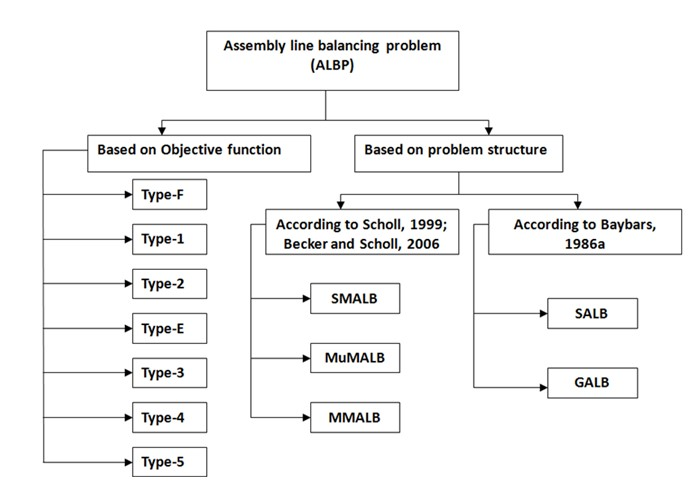
\includegraphics[width=1\linewidth]{fig/Screenshot_1.jpg}}
    \caption{Классификация ALBP}
    \label{ris:image1}
\end{figure}

\subsection{Проблемы базирующиеся на целевых функциях}
В данном подразделе рассматриваются целевые задачи балансировки линии. Далее перечисленные все обозримые проблемы приведенные на классификации \ref{ris:image1} и представленно их краткое описание.
\begin{itemize}
    \item Type F: Рассматривает возможность создание линии при заданном колличестве рабочих станций и цикле.
    \item Type 1: Рассматривает задачу минимизации количества рабочих станций, при фиксированном времени цикла.
    \item Type 2: Рассматривает задачу минимизации времени цикла, при фиксированном количестве рабочих станций.
    \item Type E: Данный тип является самой общей версией ПРТ и рассматривает получение максимальной эффективности линии при минимальном цикле и количестве станций.
    \item Type 3: Рассматривает задачу максимизации плавности рабочей нагрузки.
    \item Type 4: Рассматривают максимизацию рабочей связанности, используется для быстрого производства однотипного продукта.
    \item Type 5: Рассматривает типы 3 и 4 для нескольких продуктов
\end{itemize}

В рамках данной работы рассматривается функция повышения эффективности загрузки. Эффективность сборочной линии подразумевает равную загрузку всех рабочих станций на сборочной линии. 

\subsection{Проблемы основывающиеся на структуре линии}
В данном разделе рассматриваются структурные задачи балансировки линии. Далее перечислены структурные проблемы приведенные на рисунке (\ref{ris:image1}) и их описание.

\begin{itemize}
    \item SMALB: Данная проблема затрагивает структуру, когда на линии производится один тип продукта
    \item MuMALBP: Затрагивает проблемы производства более одного типа продукта партиями на одной линии
    \item MMALBP: Затрагивает производство разных типов продуктов на одной линии в любом порядке, без времени переключения (имется ввиду переключение на производство другого типа продукта)
\end{itemize}

\begin{figure}[H]
    \center{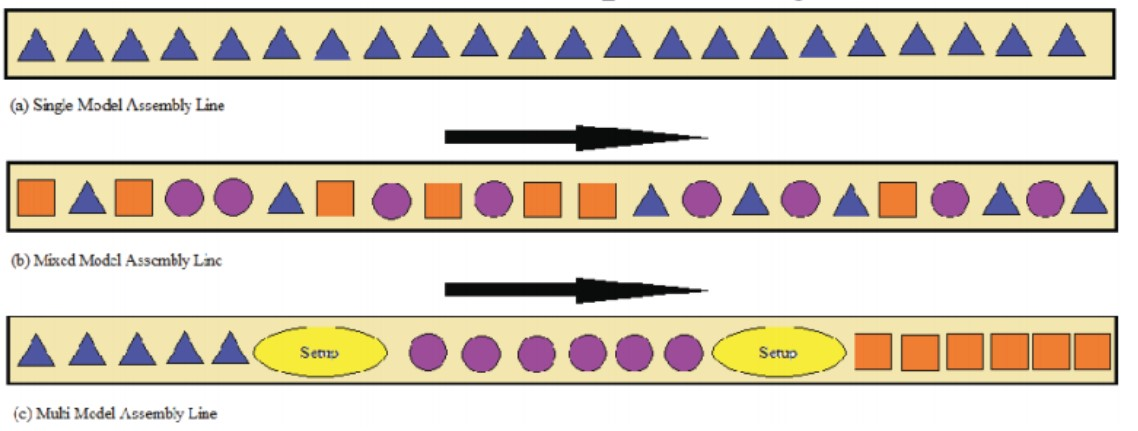
\includegraphics[width=1\linewidth]{fig/Screenshot_2.jpg}}
    \caption{Структура линий из классификации, изображенной на рисунке \ref{ris:image1}}
    \label{ris:shapeOfLines}
\end{figure}

Созданная имитационная модель позволяет игнорировать структурные особенности линии. Основные ограничения, которые невозможно игнорировать включены в технологическую карту. 
\todo[inline, color=red]{Пока непонятно куда девать время предустановки линии в случае MMALBP}

Источник: https://ru.scribd.com/doc/7699063/Introduction-of-Line-Balancing



\section{Обзоры методов решения проблем балансировки линии}

На текущий момент известны множество подходов решения проблемы балансировки линии. Наиболее популярные подходы и методы приведены на рисунке (\ref{ris:Approaches}).

\begin{figure}[H]
    \center{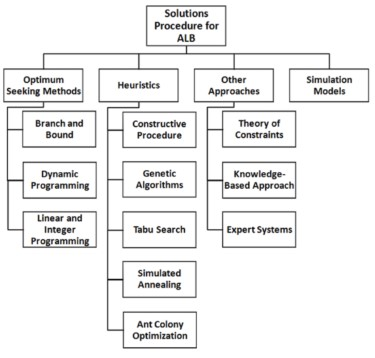
\includegraphics[width=1\linewidth]{fig/Approaches.jpg}}
    \caption{Различные процедуры решения для ALB}
    \label{ris:Approaches}
\end{figure}

Методы оптимального поиска основаны на математических подходах и позволяют найти из множества объектов оптимальный, который соответствует заданным критериям. Одной из основных проблем данного подхода является вычислительная сложность, что в контексте поиска наилучшей конфигурации конвейера, приводит к существенному ограничению использования методов оптимального поиска.

Методы эвристики позволяют избежать проблемы комбинаторной сложности задачи, но при этом результат не всегда будет являться самым оптимальным из возможных. Также эффективность работы алгоритмов эвристики во многом зависят от подхода. На рисунке (\ref{ris:Approaches}) приведены 5 различных эвристических алгоритмов, которые использовались для решения проблемы балансировки линии. Наиболее эффективным из данной группы показал себя генетический алгоритм поиска(ссылка на пруфы). Рассмотрим подробно, как работает генетический алгоритм в контексте балансировки линии.

\subsection{Генетический алгоритм}

Генетические алгоритмы хорошо подходят для решения задач планирования производства, потому что в отличие от эвристических методов генетические алгоритмы работают на совокупности решений, а не на одном решении. В производственном планировании эта совокупность решений состоит из множества ответов, которые могут иметь разные, иногда противоречивые цели. Например, в одном решении оптимизировать производственный процесс, который будет завершен за минимальное время. В другом решении оптимизировать для минимального количества дефектов.

По мере того как увеличиваются количество целей, которые пытаемся достичь, также увеличивается количество ограничений на проблему и аналогичным образом увеличиваем сложность. Генетические алгоритмы идеальны для задач такого типа, когда пространство поиска велико, а количество возможных решений мало.

Чтобы применить генетический алгоритм к задаче планирования, необходимо сначала представить каким образом обозначить геном. Одним из способов представления генома планирования является определение последовательности задач и времени начала этих задач относительно друг друга. Каждое задание и соответствующее время его запуска представляют собой ген.

Определенная последовательность задач и времени начала (гены) представляет один ген в нашей популяции. Чтобы убедиться, что геном является возможным решением, надо чтобы он соответствовал ограничениям приоритета. Далее генерируется начальная популяция, используя случайные времена начала в пределах ограничений предшествования. С помощью генетических алгоритмов берется начальная популяция и скрещивается, комбинируя гены с небольшим количеством случайности (мутации). Потомки этой комбинации выбираются на основе фитнес-функции, которая включает одно или много наших ограничений, таких как минимизация времени и минимизация дефектов. Данный процесс продолжаться либо в течение заранее выделенного времени, либо до тех пор, пока не найдется решение, которое соответствует минимальным критериям. В целом каждое последующее поколение будет иметь более высокую среднюю пригодность, то есть займет меньше времени с более высоким качеством, чем предыдущие поколения. При планировании задач, как и в случае с другими решениями генетического алгоритма, необходимо убедиться, что мы не выбираются недопустимые потомки, такие как отпрыски, которые нарушают наше ограничение приоритета. Также может потребоваться добавить дополнительные значения пригодности, такие как минимизация затрат; однако каждое добавляемое ограничение значительно увеличивает пространство поиска и уменьшает количество подходящих решений.



\chapter{Экспериментальная часть}
\section{Разработка программы}
\subsection{Предобработка технологических карт}
\subsection{Генерация производственного плана аосредством имитационной модели}
\subsection{Оптимизационные подходы}
\subsubsection{Метод грубой силы}
Примером оптимизации может служить случайный выбор следующей операции при планировании, данный выбор возможен только в случаях одновременного выполнения нескольких независимых операций. Таким образом достигается вариативность при котором из разных реализаций, выбирается наилучший вариант. На рисунке (\ref{ris:Force}) изображены технологическая карта продукта и два плана, который были построены в результате случайного выбора операций. Как видно из рисунка (\ref{ris:Force}) первый план является более оптимальным по времени и ресурсам, чем второй.

\begin{figure}[H]
    \center{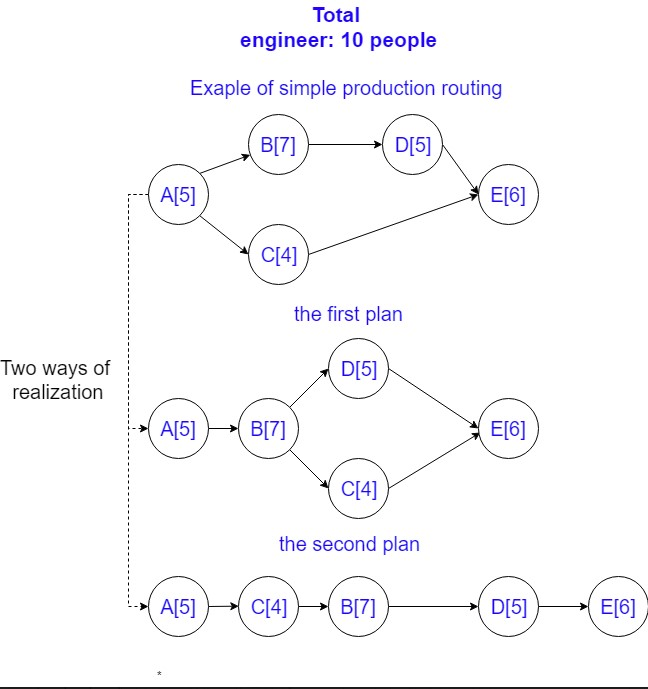
\includegraphics[width=1\linewidth]{fig/Force.jpg}}
    \caption{Два плана, полученные путем перебора исходной технологической карты}
    \label{ris:Force}
\end{figure}


\subsubsection{Частная оптимизационная задача}
\subsection{Алгоритм планирования}
Алгоритм планирования состоит из следующих этапов:
\begin{enumerate}
    \item Создание шаблона продуктов на основе заказа. Другими словами воспроизведение порядка операций указанной в технологической карте, статическая система неравенств.
    \item Создание плана на основе заказа. На данном этапе алгоритм создает шаблоны всех продуктов, которые перечислены в заказе, также учитывая количество одноименной продукции.
    \item Пошаговая реализация плана с учетом ресурсных ограничений. Добавление дополнительных ограничений в систему неравенств, которые динамически меняются с каждым шагом планирования.
\end{enumerate}
Работа имитационного моделирования представлена на рисунке \ref{ris:alg}
\begin{figure}[H]
    \center{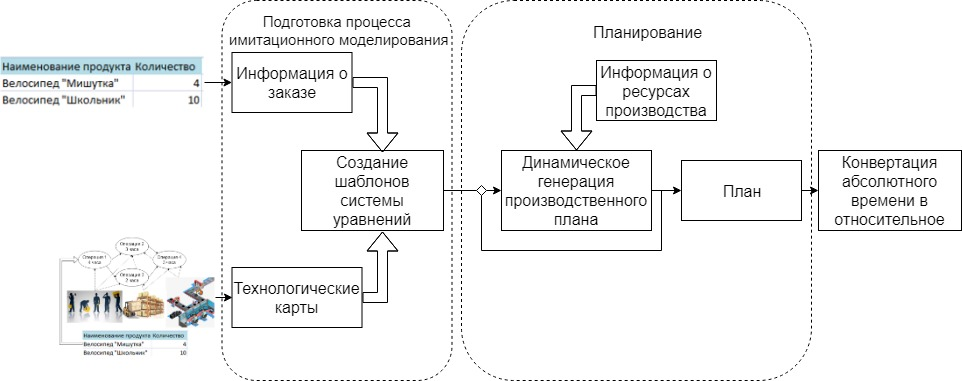
\includegraphics[width=1\linewidth]{fig/alg.jpg}}
    \caption{Визаулизация работы имитацонного моделирования}
    \label{ris:alg}
\end{figure}
\section{Демонстрация работы}
\section{Оценка экспериментальной части}

\likechapter{Заключение}
Цель достигнута, задачи выполнены